%  BE Mini Project Report - STQA Automation Testing (LP-IV)
%  Automated Testing of an E-Commerce Website Using Selenium WebDriver
%  Based on BE_PROJECT_REPORT_FORMAT_TERM_II_LATEX_FILE.tex (SPPU format)

\documentclass[oneside,a4paper,12pt]{report}

\usepackage{graphicx}
\usepackage{fancyhdr}
\usepackage{titlesec}
\usepackage{listings}
\usepackage{xcolor}
\usepackage{amsmath}
\usepackage[a4paper,margin=1in]{geometry}

\fancypagestyle{plain}{%
  \fancyhf{}
  \fancyfoot[C]{NBN SSOE, Department of Computer Engineering 2026-27}
  \fancyfoot[R]{\thepage}
}
\pagestyle{fancy}
\fancyhead{}
\renewcommand{\headrulewidth}{0pt}
\footskip = 0.625in
\cfoot{}
\rfoot{}

\usepackage[hidelinks]{hyperref}
\usepackage{tikz}
\usetikzlibrary{arrows,shapes,snakes,automata,backgrounds,petri,positioning,calc,fit}

\usepackage{tabularx}
\usepackage[nottoc,notlot,notlof,numbib]{tocbibind}
\usepackage[titletoc]{appendix}
\renewcommand{\appendixname}{Annexure}
\usepackage{titletoc}
\renewcommand{\bibname}{References}
\setcounter{secnumdepth}{5}
\usepackage{float}
\usepackage{subcaption}
\usepackage{multirow}
\usepackage[ruled,vlined]{algorithm2e}

\newcommand{\frontmatter}{\clearpage\pagenumbering{roman}}
\newcommand{\mainmatter}{\clearpage\pagenumbering{arabic}\setcounter{page}{1}}

\lstset{basicstyle=\ttfamily\footnotesize, breaklines=true, frame=single,
  columns=fullflexible, keepspaces=true, showstringspaces=false,
  keywordstyle=\color{blue}, commentstyle=\color{gray}, stringstyle=\color{red!60!black}}

\newcommand{\ptitle}{Automated Testing of an E-Commerce Website Using Selenium WebDriver}
\newcommand{\ptitleshort}{Automated Testing of an E-Commerce Website}

\begin{document}

\setlength{\parindent}{0mm}
\begin{center}

\includegraphics[width=70pt]{sppulogo.jpg}\\
{\bfseries SAVITRIBAI PHULE PUNE UNIVERSITY \\}
 \vspace*{1\baselineskip}
{\bfseries A  MINI PROJECT REPORT ON \\}
 \vspace*{2\baselineskip}
{\bfseries \fontsize{16}{12} \selectfont \ptitle \\ \vspace*{2\baselineskip}}
{\fontsize{12}{12} \selectfont SUBMITTED TOWARDS THE
 \\PARTIAL FULFILLMENT OF THE REQUIREMENTS OF \\
 LABORATORY PRACTICE IV (SOFTWARE TESTING AND QUALITY ASSURANCE)\\
\vspace*{2\baselineskip}}
{\bfseries \fontsize{14}{12} \selectfont BACHELOR OF ENGINEERING (Computer
Engineering) \\
\vspace*{1\baselineskip}}
{\bfseries \fontsize{14}{12} \selectfont BY \\
\vspace*{1\baselineskip}}
Vishwajeet Tulse  \hspace{25 mm} Exam No: \underline{\hspace{25mm}}  \\
Student Name 2 \hspace{25 mm} Exam No: \underline{\hspace{25mm}}   \\
Student Name 3 \hspace{25 mm} Exam No: \underline{\hspace{25mm}}  \\
Student Name 4 \hspace{25 mm} Exam No: \underline{\hspace{25mm}}\\
\vspace*{2\baselineskip}
{\bfseries \fontsize{14}{12} \selectfont Under The Guidance of \\
\vspace*{1\baselineskip}}
Prof. Guide Name\\
\vspace*{1\baselineskip}

\includegraphics[width=100pt]{SinhgadLogo.jpg} \\
{\bfseries \fontsize{14}{12} \selectfont DEPARTMENT OF COMPUTER ENGINEERING \\
NBN SINHGAD SCHOOL OF ENGINEERING \\
10/1, AMBEGAON (BK), PUNE-411041 \\
2026-27
}
\end{center}

\newpage

\begin{figure}[ht]
\centering

\includegraphics[width=100pt]{SinhgadLogo.jpg}
\end{figure}

{\bfseries \fontsize{14}{12} \selectfont \centerline{NBN SINHGAD SCHOOL OF ENGINEERING}
\centerline{DEPARTMENT OF COMPUTER ENGINEERING}
\vspace*{2\baselineskip}}

{\bfseries \fontsize{16}{12} \selectfont \centerline{CERTIFICATE}
\vspace*{2\baselineskip}}

\centerline{This is to certify that the Mini Project Entitled}
\vspace*{.5\baselineskip}

{\bfseries \fontsize{14}{12} \selectfont \centerline{\ptitleshort}
\vspace*{0.5\baselineskip}}

\centerline{Submitted by}
\vspace*{0.5\baselineskip}
\centerline{Vishwajeet Tulse  \hspace{25 mm} Exam No: \underline{\hspace{25mm}} }
\centerline{Student Name 2 \hspace{25 mm} Exam No: \underline{\hspace{25mm}}  }
\centerline{Student Name 3 \hspace{25 mm} Exam No: \underline{\hspace{25mm}} }
\centerline{Student Name 4 \hspace{25 mm} Exam No: \underline{\hspace{25mm}} }
\vspace*{0.5\baselineskip}

is a bonafide work carried out by Students under the supervision of Prof. Guide Name and it
is submitted towards the partial fulfillment of the requirement of Bachelor of Engineering (Computer Engineering) for the course Laboratory Practice IV.\\

\bgroup
\def\arraystretch{0.7}
\vspace*{0.5\baselineskip}
\begin{tabular}{c c }
Prof. Guide Name &  \hspace{50 mm} Dr. S. P. Bendale \\
Internal Guide   &  \hspace{50 mm} H.O.D \\
Dept. of Computer Engg.  &	\hspace{50 mm}Dept. of Computer Engg.  \\
\end{tabular}
\egroup
\vspace*{0.5\baselineskip}
\begin{center}
{
Dr. S. P. Patil \\
Principal\\
NBN Sinhgad School of Engineering
}
\end{center}
\vspace*{1\baselineskip}
Signature of Internal Examiner \hspace{30 mm} Signature of External Examiner
\newpage

\begin{center}
\textbf{PROJECT APPROVAL SHEET}
\end{center}
\begin{center}
 \ptitle
 \end{center}
\begin{center}
Is successfully completed by
\end{center}
\centerline{Vishwajeet Tulse  \hspace{25 mm} Exam No: \underline{\hspace{25mm}} }
\centerline{Student Name 2 \hspace{25 mm} Exam No: \underline{\hspace{25mm}}  }
\centerline{Student Name 3 \hspace{25 mm} Exam No: \underline{\hspace{25mm}} }
\centerline{Student Name 4 \hspace{25 mm} Exam No: \underline{\hspace{25mm}} }
\begin{center}
 at
 \end{center}
 \begin{center}
 DEPARTMENT OF COMPUTER ENGINEERING
 \end{center}
 \begin{center}
 NBN SINHGAD SCHOOL OF ENGINEERING, PUNE
 \end{center}
 \begin{center}
 SAVITRIBAI PHULE PUNE UNIVERSITY, PUNE
 \end{center}
 \begin{center}
 ACADEMIC YEAR 2026-2027
 \end{center}
 \vspace*{1\baselineskip}
 \begin{tabular}{c c }
Prof. Guide Name &  \hspace{50 mm} Dr. S. P. Bendale \\
Internal Guide   &  \hspace{50 mm} H.O.D \\
Dept. of Computer Engg.  &	\hspace{50 mm}Dept. of Computer Engg.  \\
\end{tabular}
\newpage

\setcounter{page}{0}
\frontmatter
\cfoot{NBN SSOE, Department of Computer Engineering 2026-27}
\rfoot{\thepage}
\pagenumbering{Roman}

{  \newpage {\bfseries \fontsize{14}{12} \selectfont \centerline{Abstract}
\vspace*{2\baselineskip}} \setlength{\parindent}{11mm} }
{ \setlength{\parindent}{0mm} }
Every change to a web application risks breaking features that already worked. Running the same manual test cases again after every change is slow and error-prone, which is why stable, repeatable test cases are automated. This mini project builds an automated regression test suite for \textbf{Swag Labs} (\url{https://www.saucedemo.com}), a public demo e-commerce website with login, product catalogue, shopping cart and checkout, using \textbf{Selenium WebDriver} driven from \textbf{Python} with the \textbf{pytest} framework.

The passing test cases from the companion manual-testing project were selected for automation. The suite is organised with a light Page Object Model: four small classes (\texttt{LoginPage}, \texttt{InventoryPage}, \texttt{CartPage}, \texttt{CheckoutPage}) hold the element locators and user actions of each page, so that tests read like user stories and locator changes are confined to one file. A pytest fixture starts a fresh headless Microsoft Edge browser for every test and closes it afterwards; a hook captures a screenshot whenever a test fails and embeds it in a self-contained HTML report produced by pytest-html. Parametrisation is used to run the same login and checkout validation logic with several data sets, and a known defect of the \texttt{problem\_user} account is kept in the suite as an expected failure so that the day it is fixed the suite will report it.

The final suite contains 22 test functions across five modules (login, products, cart, checkout, navigation). A full run in headless Edge takes about 105 seconds and the latest execution reports 21 passed and 1 expected failure. The project demonstrates locator strategies (ID, class name, CSS selector), explicit waits, test fixtures, data-driven tests, reporting and failure diagnosis, which are the core skills of Selenium-based test automation taught in the Software Testing and Quality Assurance course.

{  \newpage {\bfseries \fontsize{14}{12} \selectfont \centerline{Acknowledgments}
\vspace*{2\baselineskip}} \setlength{\parindent}{11mm} }
{ \setlength{\parindent}{0mm} }
\textit{It gives us great pleasure in presenting the mini project report
on {\bfseries \fontsize{12}{12} \selectfont `\ptitleshort'}.}
\vspace*{1.5\baselineskip}

 \textit{We would like to take this opportunity to thank our internal guide
 \textbf{Prof. Guide Name} for giving us all the help and guidance we needed. We are
 really grateful to them for their kind support. Their valuable suggestions were very helpful.} \vspace*{1.5\baselineskip}

 \textit{We are also grateful to \textbf{Dr. S. P. Bendale}, Head of Computer
 Engineering Department, NBN Sinhgad School of Engineering, for his indispensable
 support and suggestions.}
\vspace*{1.5\baselineskip}

\textit{In the end our special thanks to the \textbf{laboratory staff of the Department of Computer Engineering} for
providing various resources such as the laboratory with all needed software platforms and
continuous Internet connection for our project.}
\vspace*{3\baselineskip} \\
\begin{tabular}{p{8.2cm}c}
&Vishwajeet Tulse\\
&Student Name 2\\
&Student Name 3\\
&Student Name 4\\
&(B.E. Computer Engg.)
\end{tabular}

\tableofcontents
\listoffigures
\listoftables

\mainmatter

\titleformat{\chapter}[display]
{\fontsize{16}{15}\filcenter}
{\vspace*{\fill}
 \bfseries\LARGE\MakeUppercase{\chaptertitlename}~\thechapter}
{1pc}
{\bfseries\LARGE\MakeUppercase}
[\thispagestyle{empty}\vspace*{\fill}\newpage]

\setlength{\parindent}{11mm}

% =====================================================================
\chapter{Synopsis}

\section{Project Title}
\ptitle

\section{Project Option}
Internal project (mini project for Laboratory Practice IV, Software Testing and Quality Assurance).

\section{Internal Guide}
Prof. Guide Name

\section{Sponsorship and External Guide}
Not applicable. The project is not sponsored.

\section{Technical Keywords (As per ACM Keywords)}
\begin{enumerate}
  \item Software and its engineering
  \begin{enumerate}
    \item Software verification and validation
    \begin{enumerate}
      \item Software testing and debugging
      \item Regression testing, test automation
    \end{enumerate}
    \item Software notations and tools
    \begin{enumerate}
      \item Scripting languages (Python), testing frameworks
    \end{enumerate}
  \end{enumerate}
  \item Information systems
  \begin{enumerate}
    \item Web applications, electronic commerce
  \end{enumerate}
\end{enumerate}

\section{Problem Statement}
\label{sec:problem}
Design and implement an automated functional regression test suite for an e-commerce website (Swag Labs) using Selenium WebDriver, covering login, product listing and sorting, shopping cart, checkout and navigation, with reusable page objects, data-driven test cases, automatic screenshots on failure and an HTML execution report.

\section{Abstract}
\begin{itemize}
  \item Manual regression testing of a web shop after every release is slow and repetitive; automation makes it fast and repeatable.
  \item Selenium WebDriver drives a real browser through the W3C WebDriver protocol, so tests exercise the application exactly as a user would.
  \item The suite uses Python, pytest and a Page Object Model; 22 tests cover five modules.
  \item Fixtures give every test a fresh browser; a hook captures screenshots on failure; pytest-html produces a single report file.
  \item The latest run: 21 passed, 1 expected failure (a documented site defect), in about 105 seconds.
\end{itemize}

\section{Goals and Objectives}
\begin{itemize}
  \item To set up Selenium WebDriver with Python and a browser driver on Windows.
  \item To automate the stable test cases of the Swag Labs purchase flow.
  \item To apply the Page Object Model so that tests are readable and maintainable.
  \item To use pytest fixtures, parametrisation and markers (xfail) effectively.
  \item To generate an HTML report with screenshots of failures.
  \item To keep the code small and easy to explain.
\end{itemize}

\section{Relevant mathematics associated with the Project}
\label{sec:math}
System Description:
\begin{itemize}
\item \textbf{Input:} test suite $S = \{t_1, \dots, t_{22}\}$; browser $b$; the live application $A$; test data sets $D_i$ for parametrised tests.
\item \textbf{Output:} verdict $v: S \rightarrow \{\mathrm{pass}, \mathrm{fail}, \mathrm{xfail}\}$; HTML report; screenshot set for failed tests.
\item \textbf{Data structures:} locator tuples $(by, value)$; page object classes; pytest fixture graph; lists of product names and prices used in sort assertions.
\item \textbf{Functions:}
  \begin{itemize}
    \item $setup: b \rightarrow driver$ (fixture), $teardown: driver \rightarrow \emptyset$.
    \item $action: (page, input) \rightarrow page'$ (click, type, select).
    \item $assert: observed = expected$; e.g. for sorting, $prices = \mathrm{sort}(prices)$; for checkout, $total = subtotal + \mathrm{round}(0.08 \cdot subtotal, 2)$.
  \end{itemize}
\item \textbf{Mathematical formulation:} Each test is a predicate $P_i(A)$; the suite passes iff $\bigwedge_i P_i(A)$ holds for all tests not marked xfail. Running time $T = \sum_i (t_{setup} + t_{actions,i})$, about 105 s for 22 tests, versus roughly 2 hours for the same cases by hand.
\item \textbf{Success Conditions:} browser driver starts; application reachable; all assertions hold; report generated.
\item \textbf{Failure Conditions:} element not found (locator changed), timeout (slow page), assertion failure (defect); each produces a screenshot.
\end{itemize}

\section{Names of Conferences / Journals where papers can be published}
\begin{itemize}
\item IEEE International Conference on Software Testing, Verification and Validation (ICST)
\item ACM International Symposium on Software Testing and Analysis (ISSTA)
\item International Workshop on Automation of Software Test (AST)
\item SPPU-sponsored and IIT-hosted student technical conferences / workshops
\end{itemize}

\section{Review of Conference/Journal Papers supporting Project idea}
\label{sec:survey}
\begin{enumerate}
  \item Garousi and M\"antyl\"a \cite{garousi2016} review when test automation pays off: stable, repeated, regression-type tests, which is exactly our selection criterion.
  \item Leotta et al. \cite{leotta2013,leotta2014} measure the maintenance benefit of the Page Object pattern and compare locator strategies, motivating our design.
  \item Bruns, Kornstadt and Wichmann \cite{bruns2009} describe web application testing with Selenium in practice.
  \item Ramya, Sindhura and Sagar \cite{ramya2017} compare automation tools and recommend Selenium for web GUIs.
  \item Rafi et al. \cite{rafi2012} summarise benefits and limitations of automation found in a systematic review.
  \item Berner, Weber and Keller \cite{berner2005} give lessons learned on keeping automated suites maintainable.
  \item The Selenium \cite{seleniumdocs} and pytest \cite{pytestdocs} documentation define the APIs used.
  \item Pressman \cite{bookPressman} supplies the project-planning and risk framework.
\end{enumerate}

\section{Plan of Project Execution}
Four weeks: (1) environment setup and study of Selenium/pytest, (2) page objects and login/products tests, (3) cart, checkout and navigation tests, reporting and screenshots, (4) full runs, repository and report. See Annexure C.

% =====================================================================
\chapter{Technical Keywords}
\section{Area of Project}
Software Testing and Quality Assurance: automated functional and regression testing of web applications.

\section{Technical Keywords}
\begin{enumerate}
  \item Software and its engineering
  \begin{enumerate}
    \item Software testing and debugging; regression testing; test automation
    \item Software design patterns (Page Object Model)
  \end{enumerate}
  \item Information systems
  \begin{enumerate}
    \item Web applications; browsers; electronic commerce
  \end{enumerate}
  \item Computing methodologies
  \begin{enumerate}
    \item Scripting languages (Python)
  \end{enumerate}
\end{enumerate}

% =====================================================================
\chapter{Introduction}
\section{Project Idea}
\begin{itemize}
\item Convert the stable test cases of a web shop into Selenium scripts that a computer can run in minutes, every time the application changes.
\item Keep the design simple: one Page Object class per page, one test file per module, one fixture that opens and closes the browser, one command to run everything and get a report.
\item Use the public Swag Labs demo so that no server setup is needed and the suite can be run anywhere.
\end{itemize}

\section{Motivation of the Project}
\begin{itemize}
\item Regression suites are executed many times; automation turns a two-hour manual run into a two-minute unattended run.
\item Selenium WebDriver is the industry-standard open-source tool for browser automation and is part of the LP-IV syllabus (Assignment 10).
\item The companion manual-testing project produced a set of well-defined test cases with known expected results, which is the ideal input for automation.
\end{itemize}

\section{Literature Survey}
\begin{itemize}
\item \textbf{Garousi and M\"antyl\"a (2016)} \cite{garousi2016}: multi-vocal review on when and what to automate; recommends automating stable regression tests and keeping exploratory tests manual. Our suite automates only cases that passed manually.
\item \textbf{Leotta et al. (2013)} \cite{leotta2013}: industrial case study showing that Page Object based Selenium suites need far less maintenance effort when the application changes than scripts with inline locators.
\item \textbf{Leotta et al. (2014)} \cite{leotta2014}: compares ID-based and XPath locators; ID locators are more robust, which is why the suite uses IDs wherever the application provides them.
\item \textbf{Bruns, Kornstadt and Wichmann (2009)} \cite{bruns2009}: early experience report on Selenium for web application testing, including the need for waits and stable test data.
\item \textbf{Ramya, Sindhura and Sagar (2017)} \cite{ramya2017}: survey of automation tools (Selenium, QTP, TestComplete) concluding Selenium is the most suitable free tool for web applications.
\item \textbf{Rafi et al. (2012)} \cite{rafi2012}: systematic literature review on benefits (reusability, repeatability, cost over time) and limitations (initial effort, maintenance) of test automation.
\item \textbf{Berner, Weber and Keller (2005)} \cite{berner2005}: lessons from industrial automation projects: keep tests independent, make failures diagnosable (our screenshot hook), run often.
\item \textbf{Selenium documentation} \cite{seleniumdocs}: WebDriver API, locator strategies, waits, Page Object pattern.
\item \textbf{pytest documentation} \cite{pytestdocs}: fixtures, parametrisation, markers, hooks; pytest-html plugin for reports.
\item \textbf{Sauce Labs} \cite{saucedemo}: description of the Swag Labs demo and its test users.
\end{itemize}

% =====================================================================
\chapter{Problem Definition and scope}
\section{Problem Statement}
Build an automated test suite that logs in to Swag Labs, verifies the product list and sorting, adds and removes items in the cart, completes checkout with correct totals, checks form validation and navigation, and reports results with evidence, so that the whole regression run needs no human interaction.

\subsection{Goals and objectives}
\begin{itemize}
  \item Input: the application URL, test user credentials, product identifiers and test data embedded in the tests; command-line options for browser and headed/headless mode.
  \item Output: console verdicts, \texttt{reports/report.html}, screenshots of failed tests.
  \item Objective: full, unattended regression run under three minutes with clear failure diagnostics.
\end{itemize}

\subsection{Statement of scope}
\begin{itemize}
  \item In scope: functional tests of login (positive and negative), product listing and sorting, cart operations, checkout validation and totals, order completion, logout and protected-page access, in Microsoft Edge (Chrome supported by option).
  \item Out of scope: visual/pixel comparison, performance measurement, mobile browsers, tests of deliberately broken users except one documented expected failure.
\end{itemize}

\section{Major Constraints}
\begin{itemize}
  \item The application is public and may change its DOM; locators are centralised in page objects to limit the impact.
  \item Tests must be independent: each test gets a fresh browser session, so no test depends on another's cart state.
  \item Network latency varies; explicit and implicit waits are used instead of fixed sleeps.
  \item The suite must run headless on a laboratory machine without a display and without Java (Python bindings are used).
\end{itemize}

\section{Methodologies of Problem solving and efficiency issues}
\begin{itemize}
  \item \textbf{Record and playback (Selenium IDE):} quick but produces brittle scripts with duplicated locators.
  \item \textbf{Linear scripts with inline locators:} simple but every DOM change requires editing many tests.
  \item \textbf{Page Object Model with pytest (chosen):} locators and actions live in one class per page; tests are short and readable; fixtures remove setup duplication. Cost: one extra file. Efficiency: a fresh browser per test adds about 2 seconds each but guarantees isolation; the full suite runs in about 105 seconds.
\end{itemize}

\section{Outcome}
\begin{itemize}
  \item A working Selenium/pytest suite of 22 tests with page objects, fixtures, parametrisation and an xfail marker.
  \item Self-contained HTML report and screenshot-on-failure mechanism.
  \item GitHub repository with documentation and this report.
\end{itemize}

\section{Applications}
\begin{itemize}
  \item Nightly or per-commit regression testing of e-commerce sites in a CI pipeline.
  \item Smoke testing after deployment to production.
  \item Template for automating any form-based web application.
\end{itemize}

\section{Hardware Resources Required}
\begin{table}[!htbp]
\begin{center}
\def\arraystretch{1.5}
  \begin{tabular}{| c | c | c | p{5.5cm} |}
\hline
Sr. No. &	Parameter &	Minimum Requirement & Justification \\
\hline
1 &	CPU Speed &	 2 GHz dual core  & A headless browser instance per test\\
\hline
2 &	RAM  &	4 GB &  Browser plus Python interpreter\\
\hline
3 &	Network  &	Broadband Internet &  Application is hosted online\\
\hline
\end{tabular}
 \caption { Hardware Requirements }
 \label{tab:hreq}
\end{center}
\end{table}

\section{Software Resources Required}
Platform :
\begin{enumerate}
\item Operating System: Windows 11 (Linux/macOS also supported)
\item IDE: Visual Studio Code
\item Programming Language: Python 3.14 with Selenium 4.51, pytest 9, pytest-html 4
\item Browser: Microsoft Edge 142 (driver managed automatically by Selenium Manager)
\item Version control: Git and GitHub
\end{enumerate}

% =====================================================================
\chapter{Project Plan}

\section{Project Estimates}
A waterfall model was followed: requirements (select cases), design (page objects), implementation (tests), testing (runs), documentation.
\subsection{Reconciled Estimates}
\subsubsection{Cost Estimate}
All tools are free and open source. Effort about 40 person-hours for four students.

\subsubsection{Time Estimates}
\begin{table}[!htbp]
\begin{center}
\def\arraystretch{1.3}
\begin{tabular}{| l | c |}
\hline
Phase & Duration \\ \hline
Environment setup, Selenium and pytest study & 3 days \\ \hline
Page object design, login and products tests & 4 days \\ \hline
Cart, checkout, navigation tests; report and screenshot hook & 5 days \\ \hline
Full runs, debugging, code review & 2 days \\ \hline
Report and repository & 4 days \\ \hline
\textbf{Total} & \textbf{18 working days} \\ \hline
\end{tabular}
\caption{Time estimates}
\label{tab:time}
\end{center}
\end{table}

\subsection{Project Resources}
People: four students and one guide. Hardware: one laptop per student. Software: Python, Selenium, pytest, Edge, VS Code, Git/GitHub, MiKTeX.

\section{Risk Management w.r.t. NP Hard analysis}
Test execution is linear in the number of tests; no NP-hard component exists. Practical risks follow.
\subsection{Risk Identification}
Risks were identified from the questionnaire in \cite{bookPressman}: requirements (the selected manual cases) are stable; the team has Python skills; the main uncertainty is the external website and browser/driver compatibility.

\subsection{Risk Analysis}
\begin{table}[!htbp]
\begin{center}
\def\arraystretch{1.5}
\begin{tabularx}{\textwidth}{| c | X | c | c | c | c |}
\hline
\multirow{2}{*}{ID} & \multirow{2}{*}{Risk Description}	& \multirow{2}{*}{Probability} & \multicolumn{3}{|c|}{Impact} \\ \cline{4-6}
	& & &	Schedule	& Quality	& Overall \\ \hline
1	& Application DOM or behaviour changes, breaking locators	& Medium	& Medium	& High	& Medium \\ \hline
2	& Flaky tests due to timing (page not yet loaded)	& High	& Medium	& High	& High \\ \hline
3	& Browser/driver version mismatch on lab machines	& Medium	& Medium	& Low	& Medium \\ \hline
\end{tabularx}
\end{center}
\caption{Risk Table}
\label{tab:risk}
\end{table}

\begin{table}[!htbp]
\begin{center}
\def\arraystretch{1.5}
\begin{tabular}{| c | c | c |}
\hline
Probability & Value &	Description \\ \hline
High &	Probability of occurrence is &  $ > 75 \% $ \\ \hline
Medium &	Probability of occurrence is  & $26-75 \% $ \\ \hline
Low	& Probability of occurrence is & $ < 25 \% $ \\ \hline
\end{tabular}
\end{center}
\caption{Risk Probability definitions \cite{bookPressman}}
\label{tab:riskdef}
\end{table}

\begin{table}[!htbp]
\begin{center}
\def\arraystretch{1.5}
\begin{tabularx}{\textwidth}{| c | c | X |}
\hline
Impact & Value	& Description \\ \hline
Very high &	$> 10 \%$ & Schedule impact or Unacceptable quality \\ \hline
High &	$5-10 \%$ & Schedule impact or Some parts of the project have low quality \\ \hline
Medium	& $ < 5 \% $ & Schedule impact or Barely noticeable degradation in quality \\ \hline
\end{tabularx}
\end{center}
\caption{Risk Impact definitions \cite{bookPressman}}
\label{tab:riskImpactDef}
\end{table}

\subsection{Overview of Risk Mitigation, Monitoring, Management}
\begin{table}[!htbp]
\begin{center}
\def\arraystretch{1.5}
\begin{tabularx}{\textwidth}{| l | X |}
\hline
Risk ID	& 1 \\ \hline
Risk Description	& Application DOM or behaviour changes \\ \hline
Category	& Technology / external dependency \\ \hline
Source	& Public demo site maintained by a third party \\ \hline
Probability	& Medium \\ \hline
Impact	& High \\ \hline
Response	& Mitigate \\ \hline
Strategy	& All locators in \texttt{pages.py}; prefer stable ID locators; screenshot on failure shows what changed \\ \hline
Risk Status	& Mitigated \\ \hline
\end{tabularx}
\end{center}
\end{table}

\begin{table}[!htbp]
\begin{center}
\def\arraystretch{1.5}
\begin{tabularx}{\textwidth}{| l | X |}
\hline
Risk ID	& 2 \\ \hline
Risk Description	& Flaky tests due to timing \\ \hline
Category	& Technology \\ \hline
Source	& Observed in the first full run: login assertion checked the URL before navigation finished \\ \hline
Probability	& High \\ \hline
Impact	& High \\ \hline
Response	& Mitigate \\ \hline
Strategy	& Implicit wait of 5 s for elements plus an explicit \texttt{WebDriverWait} after login that waits for either the Products URL or an error message \\ \hline
Risk Status	& Occurred and resolved \\ \hline
\end{tabularx}
\end{center}
\end{table}

\begin{table}[!htbp]
\begin{center}
\def\arraystretch{1.5}
\begin{tabularx}{\textwidth}{| l | X |}
\hline
Risk ID	& 3 \\ \hline
Risk Description	& Browser/driver version mismatch \\ \hline
Category	& Development Environment \\ \hline
Source	& Different lab machines \\ \hline
Probability	& Medium \\ \hline
Impact	& Low \\ \hline
Response	& Mitigate \\ \hline
Strategy	& Selenium 4 Manager downloads the matching driver automatically; \texttt{--browser chrome} option as fallback \\ \hline
Risk Status	& Mitigated \\ \hline
\end{tabularx}
\end{center}
\end{table}

\section{Project Schedule}
\subsection{Project task set}
\begin{itemize}
  \item Task 1: Install Python, Selenium, pytest; verify a first script opens the site.
  \item Task 2: Design page objects and the driver fixture; automate login and products tests.
  \item Task 3: Automate cart, checkout and navigation tests; add parametrisation and xfail.
  \item Task 4: Add HTML report and screenshot-on-failure; run the full suite and fix flakiness.
  \item Task 5: Repository, README and project report.
\end{itemize}

\subsection{Task network}
Task 1 $\rightarrow$ Task 2 $\rightarrow$ Task 3 $\rightarrow$ Task 4 $\rightarrow$ Task 5; Task 4 reporting work was started in parallel with Task 3.

\subsection{Timeline Chart}
\begin{figure}[H]
\centering
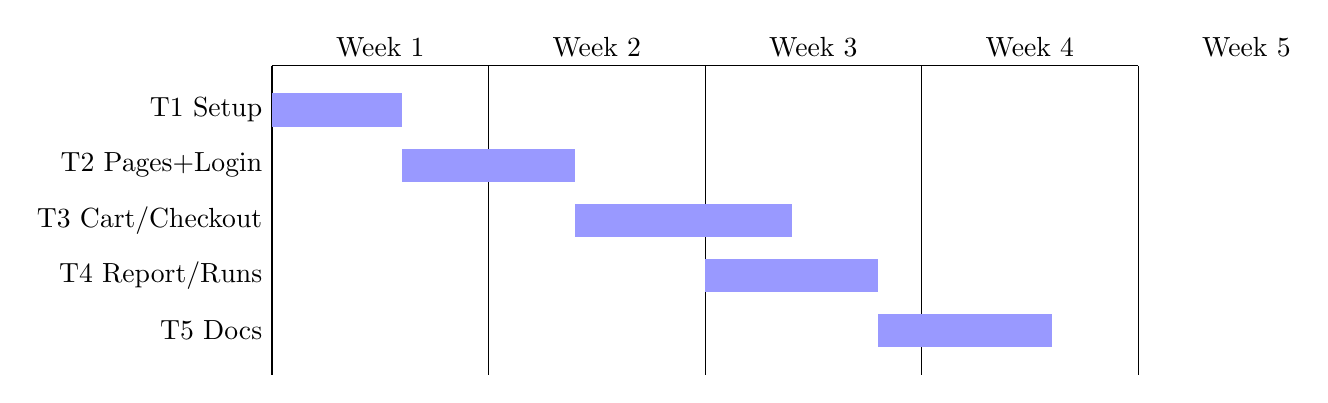
\begin{tikzpicture}[x=0.55cm,y=0.7cm]
  \foreach \w in {0,1,2,3,4} { \draw (\w*5,0.3) -- (\w*5,-5.3); \node[above] at (\w*5+2.5,0.3) {Week \the\numexpr\w+1\relax}; }
  \draw (0,0.3) -- (20,0.3);
  \node[left] at (0,-0.5) {T1 Setup};      \fill[blue!40] (0,-0.8) rectangle (3,-0.2);
  \node[left] at (0,-1.5) {T2 Pages+Login}; \fill[blue!40] (3,-1.8) rectangle (7,-1.2);
  \node[left] at (0,-2.5) {T3 Cart/Checkout}; \fill[blue!40] (7,-2.8) rectangle (12,-2.2);
  \node[left] at (0,-3.5) {T4 Report/Runs};  \fill[blue!40] (10,-3.8) rectangle (14,-3.2);
  \node[left] at (0,-4.5) {T5 Docs};       \fill[blue!40] (14,-4.8) rectangle (18,-4.2);
\end{tikzpicture}
\caption{Project timeline (Gantt chart)}
\label{fig:gantt}
\end{figure}
Please refer to Annexure C for the planner.

\section{Team Organization}
\subsection{Team structure}
Four students: one owns the framework (\texttt{conftest.py}, \texttt{pages.py}, reporting), one the login and products tests, one the cart and checkout tests, one the navigation tests, documentation and runs. Code was reviewed through GitHub commits.

\subsection{Management reporting and communication}
Weekly demonstration of the suite to the guide during the LP-IV slot; shared GitHub repository; group chat for coordination.

% =====================================================================
\chapter{Software requirement specification}

\section{Introduction}
\subsection{Purpose and Scope of Document}
This SRS states what the automated test suite must do: which features of Swag Labs it verifies, how it is run and what it produces.

\subsection{Overview of responsibilities of Developer}
Select test cases, design page objects, implement tests and fixtures, configure reporting, run and stabilise the suite, document usage.

\section{Usage Scenario}
\subsection{User profiles}
\begin{itemize}
  \item \textbf{Test engineer:} runs the suite from the command line, reads the HTML report, maintains page objects.
  \item \textbf{Developer:} runs the suite after a change to confirm nothing broke.
  \item \textbf{CI server (future):} runs the suite automatically on every commit.
\end{itemize}

\subsection{Use-cases}
\begin{table}[H]
\begin{center}
\def\arraystretch{1.5}
\begin{tabularx}{\textwidth}{| c | l | X | c | X |}
\hline
Sr No.	& Use Case	& Description	& Actors	& Assumptions \\
\hline
1& Run suite & Execute all tests headless and produce the HTML report & Test engineer & Python, Selenium and Edge installed \\
\hline
2& Run subset & Execute one module or one test by name & Test engineer & -- \\
\hline
3& Run headed & Watch the browser while tests run & Test engineer & Display available \\
\hline
4& Analyse failure & Open the report and the failure screenshot & Test engineer & A test failed \\
\hline
5& Maintain locators & Update \texttt{pages.py} after a DOM change & Test engineer & Site changed \\
\hline
6& Add test & Write a new test function using page objects & Test engineer & Page object exists \\
\hline
\end{tabularx}
\end{center}
\caption{Use Cases}
\label{tab:usecase}
\end{table}

\subsection{Use Case View}
\begin{figure}[H]
\centering
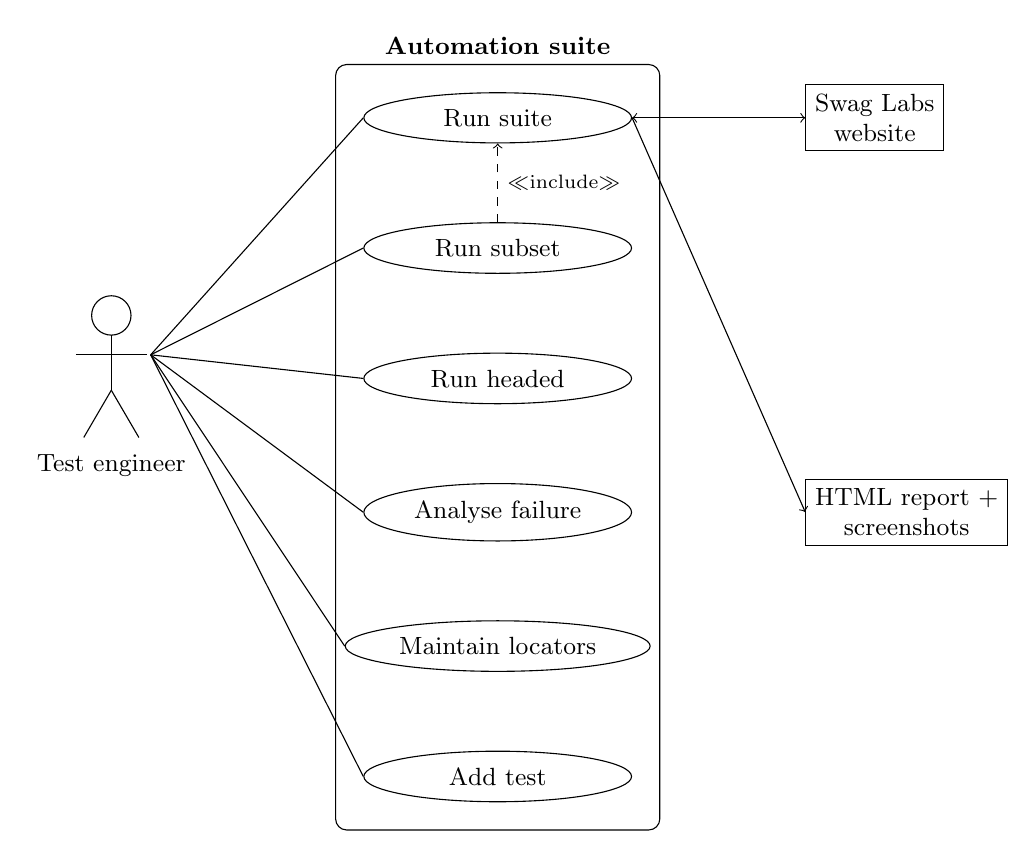
\begin{tikzpicture}[node distance=1.0cm, every node/.style={font=\small}]
  \node[draw, ellipse, minimum width=3.4cm] (u1) {Run suite};
  \node[draw, ellipse, minimum width=3.4cm, below=of u1] (u2) {Run subset};
  \node[draw, ellipse, minimum width=3.4cm, below=of u2] (u3) {Run headed};
  \node[draw, ellipse, minimum width=3.4cm, below=of u3] (u4) {Analyse failure};
  \node[draw, ellipse, minimum width=3.4cm, below=of u4] (u5) {Maintain locators};
  \node[draw, ellipse, minimum width=3.4cm, below=of u5] (u6) {Add test};
  \node[draw, rounded corners, fit=(u1)(u6), inner sep=10pt, label=above:{\textbf{Automation suite}}] (sys) {};
  \coordinate (th) at ($(u3.west)+(-3.2cm,0.8cm)$);
  \draw (th) circle (0.25);
  \draw ($(th)+(0,-0.25)$) -- ++(0,-0.7);
  \draw ($(th)+(-0.45,-0.5)$) -- ++(0.9,0);
  \draw ($(th)+(0,-0.95)$) -- ++(-0.35,-0.6);
  \draw ($(th)+(0,-0.95)$) -- ++(0.35,-0.6);
  \node at ($(th)+(0,-1.9)$) {Test engineer};
  \coordinate (tact) at ($(th)+(0.5,-0.5)$);
  \foreach \u in {u1,u2,u3,u4,u5,u6} \draw (tact) -- (\u.west);
  \node[draw, rectangle, right=2.2cm of u1, align=center] (site) {Swag Labs\\website};
  \node[draw, rectangle, right=2.2cm of u4, align=center] (rep) {HTML report +\\screenshots};
  \draw[<->] (u1.east) -- (site.west);
  \draw[->] (u1.east) -- (rep.west);
  \draw[dashed,->] (u2) -- (u1) node[midway,right] {\scriptsize $\ll$include$\gg$};
\end{tikzpicture}
\caption{Use case diagram}
\label{fig:usecase}
\end{figure}

\section{Data Model and Description}
\subsection{Data Description}
The suite holds three kinds of data: \emph{locators} (strategy, value) in the page objects; \emph{test data} (usernames, passwords, names, postal codes, expected messages) in parametrised tests; \emph{results} (verdict, duration, screenshot path) collected by pytest.

\subsection{Data objects and Relationships}
\begin{figure}[H]
\centering
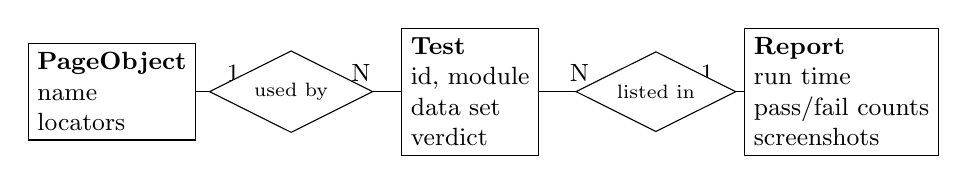
\begin{tikzpicture}[every node/.style={font=\small}]
  \node[draw, rectangle, align=left] (po) {\textbf{PageObject}\\ name\\ locators};
  \node[draw, rectangle, align=left, right=2.6cm of po] (t) {\textbf{Test}\\ id, module\\ data set\\ verdict};
  \node[draw, rectangle, align=left, right=2.6cm of t] (r) {\textbf{Report}\\ run time\\ pass/fail counts\\ screenshots};
  \draw (po) -- node[above] {1 \hspace{1.2cm} N} (t);
  \node[draw, diamond, aspect=2, fill=white, font=\scriptsize] at ($(po)!0.5!(t)$) {used by};
  \draw (t) -- node[above] {N \hspace{1.2cm} 1} (r);
  \node[draw, diamond, aspect=2, fill=white, font=\scriptsize] at ($(t)!0.5!(r)$) {listed in};
\end{tikzpicture}
\caption{Entity relationship of suite data}
\label{fig:erd}
\end{figure}

\section{Functional Model and Description}
\subsection{Data Flow Diagram}
\subsubsection{Level 0 Data Flow Diagram}
\begin{figure}[H]
\centering
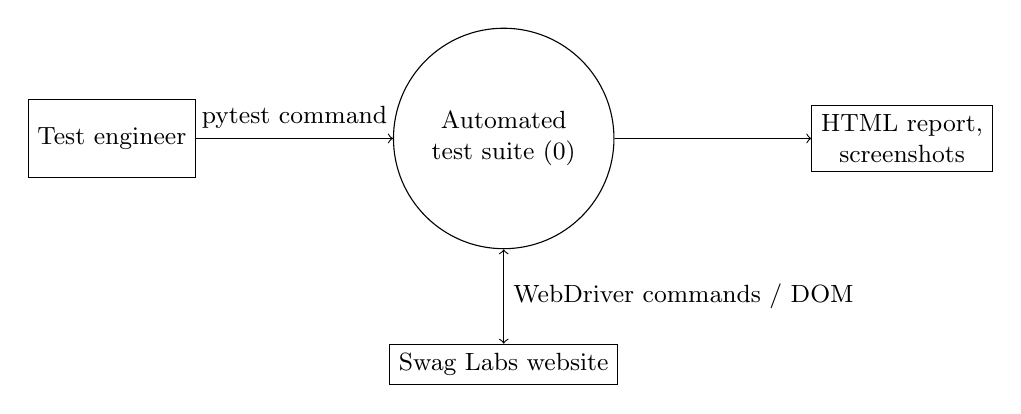
\begin{tikzpicture}[node distance=2.5cm, every node/.style={font=\small}]
  \node[draw, rectangle, minimum height=1cm] (te) {Test engineer};
  \node[draw, circle, minimum size=2.8cm, align=center, right=of te] (p) {Automated\\test suite (0)};
  \node[draw, rectangle, align=center, right=of p] (out) {HTML report,\\screenshots};
  \node[draw, rectangle, below=1.2cm of p] (app) {Swag Labs website};
  \draw[->] (te) -- node[above] {pytest command} (p);
  \draw[<->] (app) -- node[right] {WebDriver commands / DOM} (p);
  \draw[->] (p) -- (out);
\end{tikzpicture}
\caption{Level 0 DFD}
\label{fig:dfd0}
\end{figure}

\subsubsection{Level 1 Data Flow Diagram}
\begin{figure}[H]
\centering
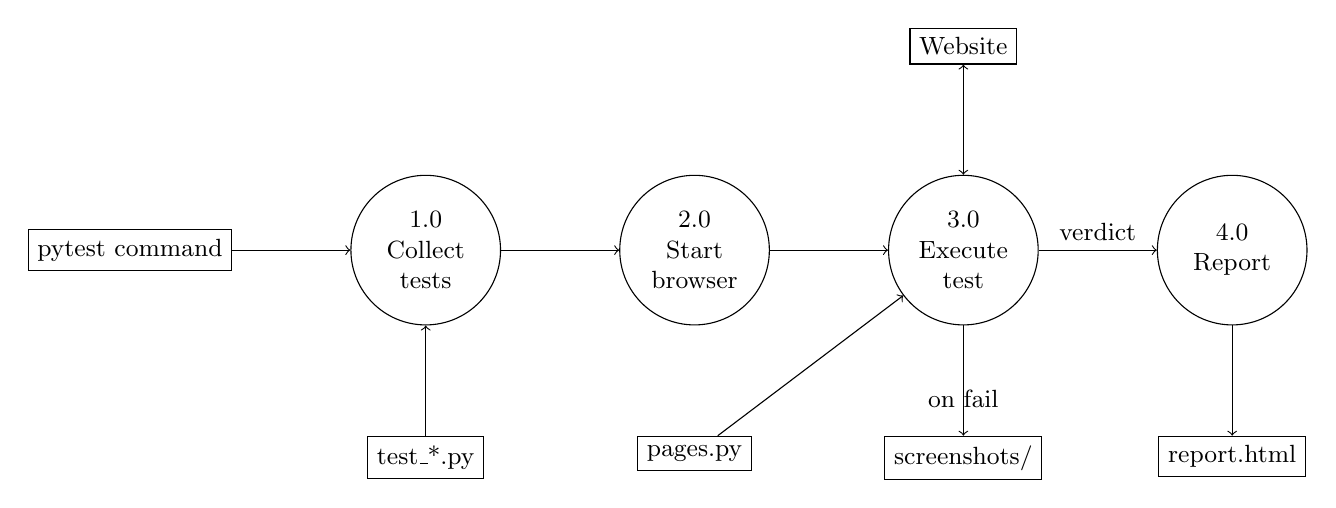
\begin{tikzpicture}[node distance=1.4cm and 1.5cm, every node/.style={font=\small}]
  \node[draw, rectangle] (cmd) {pytest command};
  \node[draw, circle, minimum size=1.9cm, align=center, right=of cmd] (p1) {1.0\\Collect\\tests};
  \node[draw, circle, minimum size=1.9cm, align=center, right=of p1] (p2) {2.0\\Start\\browser};
  \node[draw, circle, minimum size=1.9cm, align=center, right=of p2] (p3) {3.0\\Execute\\test};
  \node[draw, circle, minimum size=1.9cm, align=center, right=of p3] (p4) {4.0\\Report};
  \node[draw, rectangle, below=of p1] (files) {test\_*.py};
  \node[draw, rectangle, below=of p2] (po) {pages.py};
  \node[draw, rectangle, above=of p3] (app) {Website};
  \node[draw, rectangle, below=of p3] (shot) {screenshots/};
  \node[draw, rectangle, below=of p4] (html) {report.html};
  \draw[->] (cmd) -- (p1); \draw[->] (files) -- (p1); \draw[->] (p1) -- (p2); \draw[->] (p2) -- (p3);
  \draw[->] (po) -- (p3); \draw[<->] (p3) -- (app); \draw[->] (p3) -- node[below] {on fail} (shot);
  \draw[->] (p3) -- node[above] {verdict} (p4); \draw[->] (p4) -- (html);
\end{tikzpicture}
\caption{Level 1 DFD}
\label{fig:dfd1}
\end{figure}

\subsection{Activity Diagram:}
\begin{figure}[H]
\centering
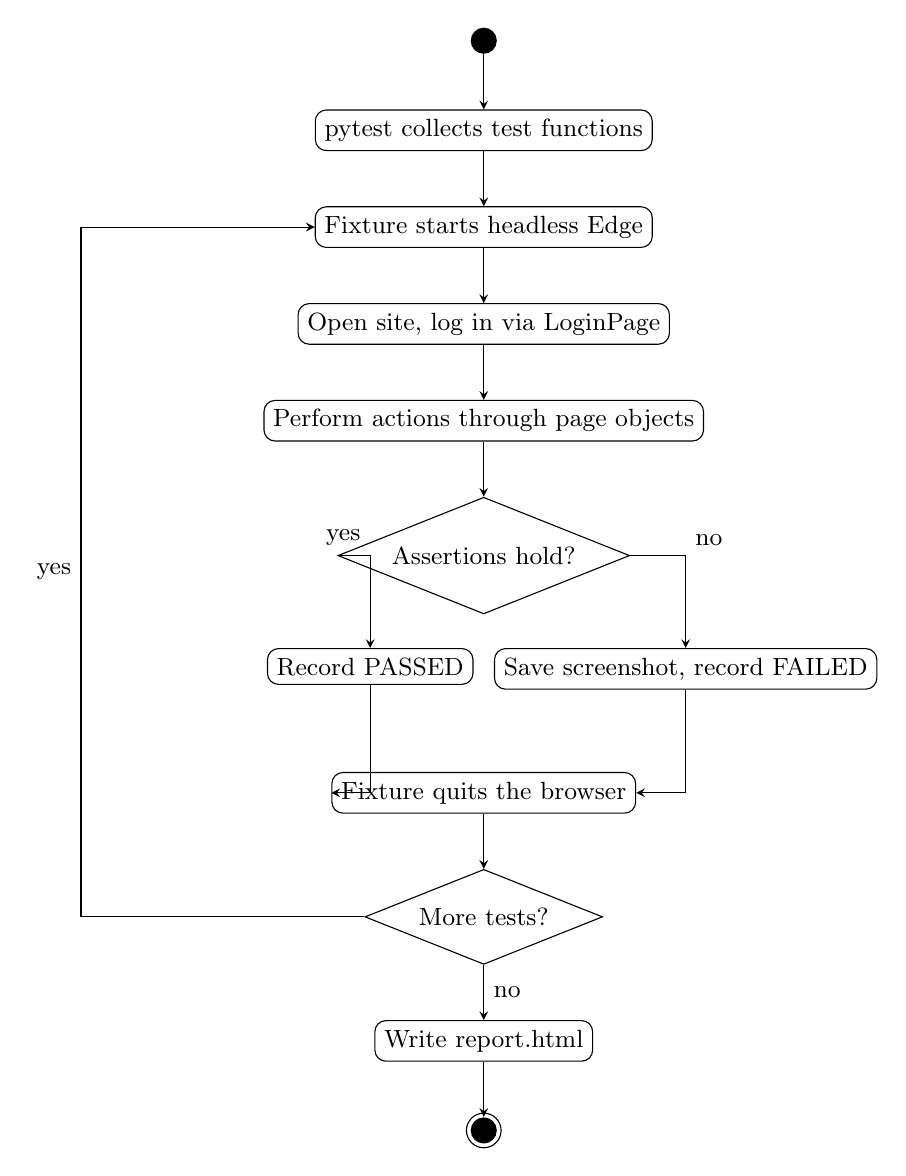
\begin{tikzpicture}[node distance=0.7cm, every node/.style={font=\small}, >=stealth]
  \node[circle, fill=black, minimum size=0.3cm] (s) {};
  \node[draw, rounded corners, below=of s] (a1) {pytest collects test functions};
  \node[draw, rounded corners, below=of a1] (a2) {Fixture starts headless Edge};
  \node[draw, rounded corners, below=of a2] (a3) {Open site, log in via LoginPage};
  \node[draw, rounded corners, below=of a3] (a4) {Perform actions through page objects};
  \node[draw, diamond, aspect=2.5, below=of a4] (d1) {Assertions hold?};
  \node[draw, rounded corners, below left=0.8cm and -0.8cm of d1] (p) {Record PASSED};
  \node[draw, rounded corners, below right=0.8cm and -0.8cm of d1] (f) {Save screenshot, record FAILED};
  \node[draw, rounded corners, below=2.0cm of d1] (q) {Fixture quits the browser};
  \node[draw, diamond, aspect=2.5, below=of q] (d2) {More tests?};
  \node[draw, rounded corners, below=of d2] (r) {Write report.html};
  \node[circle, fill=black, minimum size=0.3cm, below=of r] (e) {};
  \draw (e) circle (0.22cm);
  \draw[->] (s) -- (a1); \draw[->] (a1) -- (a2); \draw[->] (a2) -- (a3); \draw[->] (a3) -- (a4); \draw[->] (a4) -- (d1);
  \draw[->] (d1) -| node[above left] {yes} (p); \draw[->] (d1) -| node[above right] {no} (f);
  \draw[->] (p) |- (q); \draw[->] (f) |- (q);
  \draw[->] (q) -- (d2); \draw[->] (d2) -- node[right] {no} (r); \draw[->] (r) -- (e);
  \draw[->] (d2.west) -- ++(-3.6,0) |- node[pos=0.25, left] {yes} (a2.west);
\end{tikzpicture}
\caption{Activity diagram of a test run}
\label{fig:activity}
\end{figure}

\subsection{Non Functional Requirements:}
\begin{itemize}
  \item \textbf{Interface Requirements:} command line (\texttt{python -m pytest}) with options \texttt{--browser} and \texttt{--headed}; HTML report viewable in any browser.
  \item \textbf{Performance Requirements:} full suite under 3 minutes; currently about 105 s.
  \item \textbf{Reliability:} tests independent and repeatable; waits instead of sleeps.
  \item \textbf{Modifiability:} locators only in \texttt{pages.py}; tests contain no locators.
  \item \textbf{Portability:} Python and Selenium run on Windows, Linux and macOS; Edge or Chrome.
  \item \textbf{Testability / Usability:} one command runs everything; failures include a screenshot.
\end{itemize}

\subsection{State Diagram:}
Fig.\ref{fig:state-dig} shows the states of one test during execution.
\begin{figure}[H]
\centering
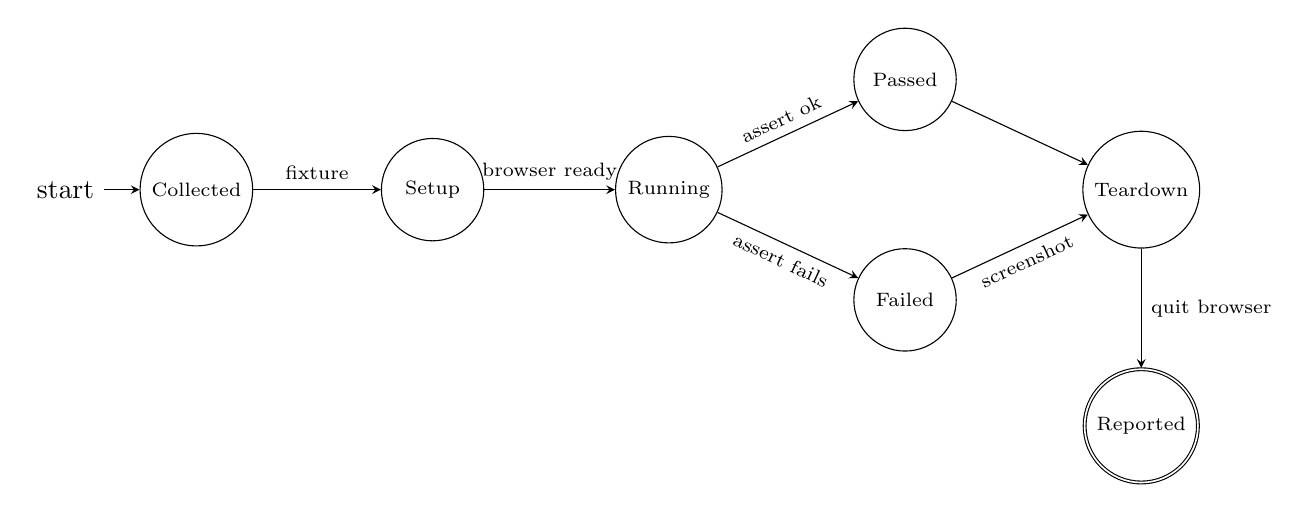
\begin{tikzpicture}[->, >=stealth, every state/.style={font=\scriptsize, minimum size=1.3cm}]
  \node[state, initial] (col) at (0,0) {Collected};
  \node[state] (setup) at (3,0) {Setup};
  \node[state] (run) at (6,0) {Running};
  \node[state] (pass) at (9,1.4) {Passed};
  \node[state] (fail) at (9,-1.4) {Failed};
  \node[state] (td) at (12,0) {Teardown};
  \node[state, accepting] (done) at (12,-3) {Reported};
  \path (col) edge node[above, font=\scriptsize] {fixture} (setup)
        (setup) edge node[above, font=\scriptsize] {browser ready} (run)
        (run) edge node[above, sloped, font=\scriptsize] {assert ok} (pass)
        (run) edge node[below, sloped, font=\scriptsize] {assert fails} (fail)
        (pass) edge (td)
        (fail) edge node[below, sloped, font=\scriptsize] {screenshot} (td)
        (td) edge node[right, font=\scriptsize] {quit browser} (done);
\end{tikzpicture}
\caption{State transition diagram of a test}
\label{fig:state-dig}
\end{figure}

\subsection{Design Constraints}
No Java (Python bindings only); no third-party page-object library; standard pytest plugins only (pytest-html).

\subsection{Software Interface Description}
\begin{itemize}
  \item \textbf{Browser interface:} Selenium WebDriver talks to msedgedriver/chromedriver over the W3C WebDriver protocol; the driver controls the browser.
  \item \textbf{Application interface:} HTTPS pages of Swag Labs.
  \item \textbf{Report interface:} pytest-html writes a self-contained HTML file; screenshots are PNG.
\end{itemize}

% =====================================================================
\chapter{Detailed Design Document using Appendix A and B}
\section{Introduction}
This chapter describes the architecture of the automation framework and its components.

\section{Architectural Design}
\begin{figure}[H]
\centering
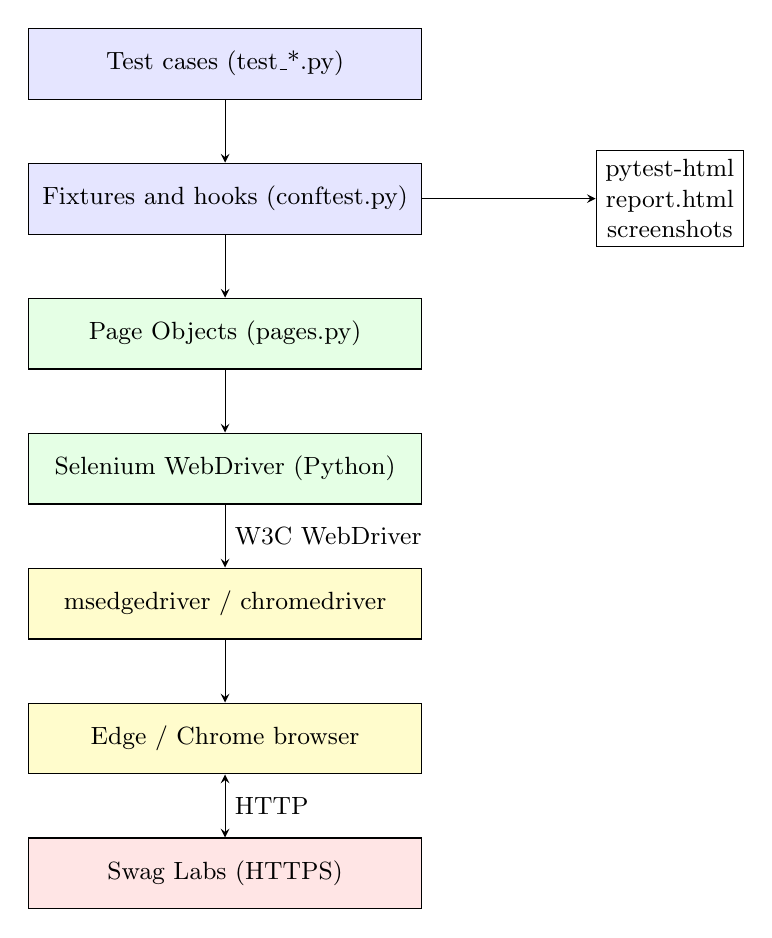
\begin{tikzpicture}[node distance=0.8cm, every node/.style={font=\small}, >=stealth]
  \node[draw, fill=blue!10, minimum width=5cm, minimum height=0.9cm] (tests) {Test cases (test\_*.py)};
  \node[draw, fill=blue!10, minimum width=5cm, minimum height=0.9cm, below=of tests] (fx) {Fixtures and hooks (conftest.py)};
  \node[draw, fill=green!10, minimum width=5cm, minimum height=0.9cm, below=of fx] (po) {Page Objects (pages.py)};
  \node[draw, fill=green!10, minimum width=5cm, minimum height=0.9cm, below=of po] (sel) {Selenium WebDriver (Python)};
  \node[draw, fill=yellow!20, minimum width=5cm, minimum height=0.9cm, below=of sel] (drv) {msedgedriver / chromedriver};
  \node[draw, fill=yellow!20, minimum width=5cm, minimum height=0.9cm, below=of drv] (br) {Edge / Chrome browser};
  \node[draw, fill=red!10, minimum width=5cm, minimum height=0.9cm, below=of br] (app) {Swag Labs (HTTPS)};
  \node[draw, right=2.2cm of fx, align=center] (rep) {pytest-html\\report.html\\screenshots};
  \draw[->] (tests) -- (fx); \draw[->] (fx) -- (po); \draw[->] (po) -- (sel); \draw[->] (sel) -- node[right] {W3C WebDriver} (drv);
  \draw[->] (drv) -- (br); \draw[<->] (br) -- node[right] {HTTP} (app);
  \draw[->] (fx) -- (rep);
\end{tikzpicture}
\caption{Architecture of the automation framework}
\label{fig:arch-dig}
\end{figure}

\section{Data design (using Appendices A and B)}
\subsection{Internal software data structure}
Locator tuples \texttt{(By.ID, "login-button")} as class attributes; lists of names and prices returned by page objects; parametrised tuples of test data.
\subsection{Global data structure}
\texttt{BASE\_URL} and \texttt{DEFAULT\_PASSWORD} in \texttt{pages.py}; \texttt{SCREENSHOT\_DIR} in \texttt{conftest.py}; command-line options \texttt{--browser}, \texttt{--headed}.
\subsection{Temporary data structure}
The WebDriver session (one per test); pytest's report objects to which screenshots are attached as extras.
\subsection{Database description}
No database. Outputs are files: \texttt{reports/report.html}, \texttt{reports/console\_output.txt}, \texttt{reports/screenshots/*.png}.

\section{Component Design}
\subsection{Class Diagram}
\begin{figure}[H]
\centering
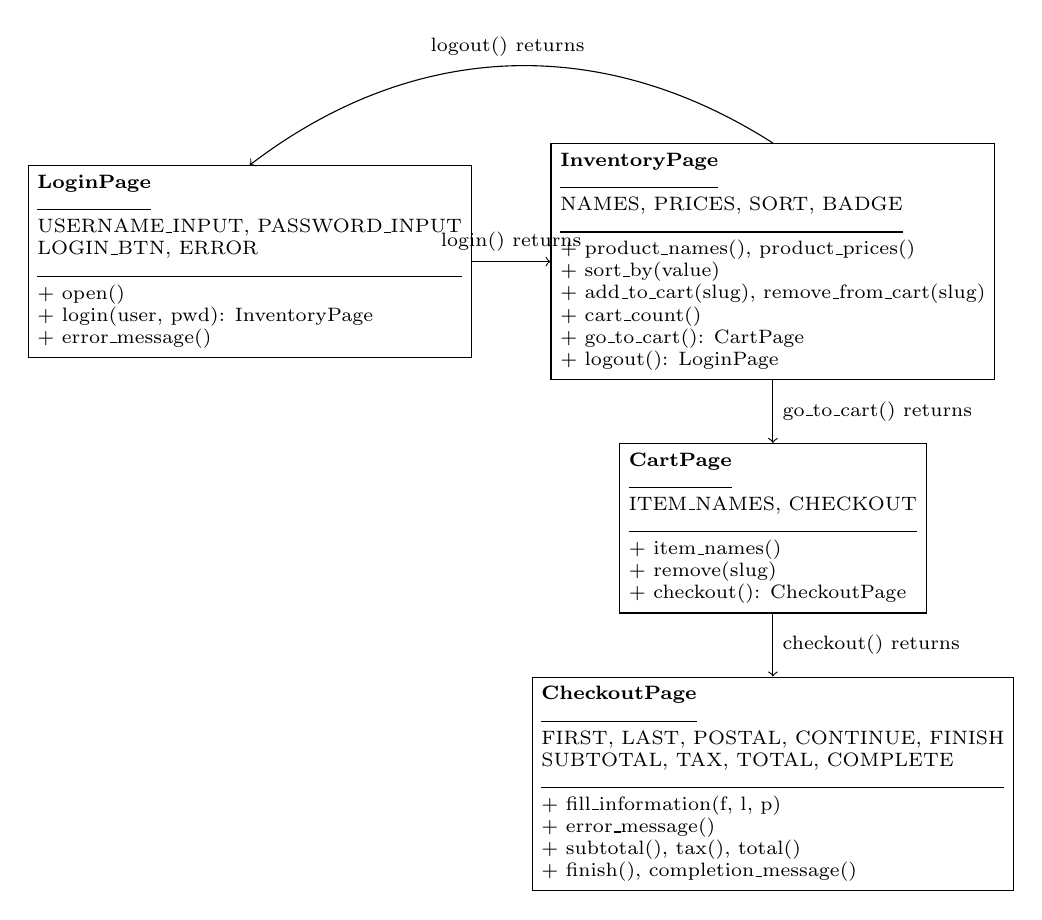
\begin{tikzpicture}[node distance=0.8cm and 1.0cm, every node/.style={font=\scriptsize}]
  \node[draw, rectangle, align=left] (lp) {\textbf{LoginPage}\\ \hrulefill\\ USERNAME\_INPUT, PASSWORD\_INPUT\\ LOGIN\_BTN, ERROR\\ \hrulefill\\ + open()\\ + login(user, pwd): InventoryPage\\ + error\_message()};
  \node[draw, rectangle, align=left, right=of lp] (ip) {\textbf{InventoryPage}\\ \hrulefill\\ NAMES, PRICES, SORT, BADGE\\ \hrulefill\\ + product\_names(), product\_prices()\\ + sort\_by(value)\\ + add\_to\_cart(slug), remove\_from\_cart(slug)\\ + cart\_count()\\ + go\_to\_cart(): CartPage\\ + logout(): LoginPage};
  \node[draw, rectangle, align=left, below=of ip] (cp) {\textbf{CartPage}\\ \hrulefill\\ ITEM\_NAMES, CHECKOUT\\ \hrulefill\\ + item\_names()\\ + remove(slug)\\ + checkout(): CheckoutPage};
  \node[draw, rectangle, align=left, below=of cp] (co) {\textbf{CheckoutPage}\\ \hrulefill\\ FIRST, LAST, POSTAL, CONTINUE, FINISH\\ SUBTOTAL, TAX, TOTAL, COMPLETE\\ \hrulefill\\ + fill\_information(f, l, p)\\ + error\_message()\\ + subtotal(), tax(), total()\\ + finish(), completion\_message()};
  \draw[->] (lp) -- node[above] {login() returns} (ip);
  \draw[->] (ip) -- node[right] {go\_to\_cart() returns} (cp);
  \draw[->] (cp) -- node[right] {checkout() returns} (co);
  \draw[->] (ip.north) to[bend right=35] node[above] {logout() returns} (lp.north);
\end{tikzpicture}
\caption{Class diagram of the page objects}
\label{fig:class-dig}
\end{figure}

% =====================================================================
\chapter{Project Implementation}
\section{Introduction}
The suite consists of \texttt{pages.py} (about 140 lines), \texttt{conftest.py} (about 60 lines) and five test files (about 120 lines in total). Repository: \url{https://github.com/VishwajeetTulse/ecommerce-automation-testing}.

\section{Tools and Technologies Used}
\begin{itemize}
  \item Python 3.14; Selenium 4.51 (WebDriver, Selenium Manager for drivers)
  \item pytest 9 (fixtures, parametrize, xfail, hooks); pytest-html 4 (report)
  \item Microsoft Edge 142 headless; Chrome optional
  \item Visual Studio Code; Git and GitHub
\end{itemize}

\section{Methodologies/Algorithm Details}
\subsection{Algorithm 1/Pseudo Code}
\begin{algorithm}[H]
\caption{Driver fixture with screenshot on failure}
\KwIn{test function $t$, options browser, headed}
\KwOut{verdict, optional screenshot}
create browser options; add \texttt{--headless=new} unless headed; set window 1280x900\;
$driver \leftarrow$ new Edge or Chrome session; implicit wait 5 s\;
run $t$ with $driver$\;
\If{$t$ failed in its call phase}{save \texttt{reports/screenshots/<test name>.png}; attach to HTML report\;}
quit $driver$\;
\end{algorithm}

\subsection{Algorithm 2/Pseudo Code}
\begin{algorithm}[H]
\caption{Checkout total verification test}
\KwIn{standard user, products Backpack (29.99) and Bike Light (9.99)}
\KwOut{pass if totals are consistent}
login; add both products; open cart; click Checkout\;
fill first name, last name, postal code; click Continue\;
$s \leftarrow$ subtotal shown; $x \leftarrow$ tax shown; $T \leftarrow$ total shown\;
assert $s = 39.98$\;
assert $x = \mathrm{round}(0.08 \cdot s, 2)$\;
assert $T = s + x$\;
\end{algorithm}

Key code: the login action with an explicit wait, and a parametrised negative test.
\begin{lstlisting}[language=Python]
def login(self, username, password=DEFAULT_PASSWORD):
    self.driver.find_element(*self.USERNAME_INPUT).send_keys(username)
    self.driver.find_element(*self.PASSWORD_INPUT).send_keys(password)
    self.driver.find_element(*self.LOGIN_BTN).click()
    # wait until either the Products page opens or an error is shown
    WebDriverWait(self.driver, 10).until(
        lambda d: "inventory.html" in d.current_url or d.find_elements(*self.ERROR))
    return InventoryPage(self.driver)

@pytest.mark.parametrize("username,password,expected", [
    ("", "", "Username is required"),
    ("standard_user", "", "Password is required"),
    ("standard_user", "wrong", "do not match any user"),
    ("locked_out_user", "secret_sauce", "locked out"),
])
def test_invalid_login_shows_error(login_page, username, password, expected):
    login_page.login(username, password)
    assert expected in login_page.error_message()
\end{lstlisting}

\section{Verification and Validation for Acceptance}
Acceptance criteria: the suite runs unattended with one command; every selected manual case has an automated equivalent; all tests pass on the current site except the documented expected failure; a failed test produces a screenshot; the HTML report is generated. All criteria were verified in the final run (Chapter 9) and by forcing the expected-failure test to run as a normal test, which produced the screenshot shown in Fig.\ref{fig:failshot}.

% =====================================================================
\chapter{Software Testing}
\section{Type of Testing Used}
\begin{itemize}
  \item \textbf{Automated functional testing} of each module through the browser (black-box, end-to-end).
  \item \textbf{Regression testing:} the full suite is re-run after any change to the tests or the site.
  \item \textbf{Data-driven testing:} parametrised login and checkout validation cases.
  \item \textbf{Testing of the framework itself:} a deliberately failing run confirmed the screenshot hook and report embedding.
\end{itemize}

\section{Test Cases and Test Results}
\begin{table}[H]
\begin{center}
\def\arraystretch{1.3}
\begin{tabularx}{\textwidth}{| l | X | c |}
\hline
Test & What is verified & Result \\ \hline
test\_valid\_login & standard\_user reaches Products page & Pass \\ \hline
test\_invalid\_login\_shows\_error [4 data sets] & empty, no password, wrong password, locked-out user show the right error & Pass (4) \\ \hline
test\_password\_is\_masked & password input type is ``password'' & Pass \\ \hline
test\_six\_products\_listed & six product names on Products page & Pass \\ \hline
test\_sort\_price\_low\_to\_high & prices ascending after sort & Pass \\ \hline
test\_sort\_price\_high\_to\_low & prices descending after sort & Pass \\ \hline
test\_sort\_name\_z\_to\_a & names in reverse alphabetical order & Pass \\ \hline
test\_sort\_price\_problem\_user & sort for problem\_user (known defect) & XFAIL \\ \hline
test\_add\_two\_items\_updates\_badge & badge shows 2 & Pass \\ \hline
test\_cart\_page\_lists\_added\_items & both items listed on cart page & Pass \\ \hline
test\_remove\_item\_from\_cart\_page & one item left, badge 1 & Pass \\ \hline
test\_remove\_from\_products\_page & badge disappears & Pass \\ \hline
test\_missing\_information\_shows\_error [3 data sets] & first name, last name, postal code required & Pass (3) \\ \hline
test\_overview\_totals\_are\_correct & subtotal 39.98, tax 8\%, total = sum & Pass \\ \hline
test\_complete\_order & ``Thank you for your order!'' page & Pass \\ \hline
test\_logout\_returns\_to\_login\_page & login page after logout & Pass \\ \hline
test\_inventory\_page\_requires\_login & direct URL shows access error & Pass \\ \hline
\end{tabularx}
\end{center}
\caption{Automated test cases and results (final run: 21 passed, 1 xfailed, 105.6 s)}
\label{tab:tests}
\end{table}

Console summary of the final run:
\begin{lstlisting}
tests/test_cart.py::test_add_two_items_updates_badge PASSED              [  4%]
tests/test_cart.py::test_cart_page_lists_added_items PASSED              [  9%]
tests/test_cart.py::test_remove_item_from_cart_page PASSED               [ 13%]
tests/test_cart.py::test_remove_from_products_page PASSED                [ 18%]
tests/test_checkout.py::test_missing_information_shows_error[---First Name is required] PASSED
tests/test_checkout.py::test_missing_information_shows_error[Vishwajeet---Last Name is required] PASSED
tests/test_checkout.py::test_missing_information_shows_error[Vishwajeet-Tulse--Postal Code is required] PASSED
tests/test_checkout.py::test_overview_totals_are_correct PASSED          [ 36%]
tests/test_checkout.py::test_complete_order PASSED                       [ 40%]
tests/test_login.py::test_valid_login PASSED                             [ 45%]
tests/test_login.py::test_invalid_login_shows_error[--Username is required] PASSED
tests/test_login.py::test_invalid_login_shows_error[standard_user--Password is required] PASSED
tests/test_login.py::test_invalid_login_shows_error[standard_user-wrong-do not match any user] PASSED
tests/test_login.py::test_invalid_login_shows_error[locked_out_user-secret_sauce-locked out] PASSED
tests/test_login.py::test_password_is_masked PASSED                      [ 68%]
tests/test_navigation.py::test_logout_returns_to_login_page PASSED       [ 72%]
tests/test_navigation.py::test_inventory_page_requires_login PASSED      [ 77%]
tests/test_products.py::test_six_products_listed PASSED                  [ 81%]
tests/test_products.py::test_sort_price_low_to_high PASSED               [ 86%]
tests/test_products.py::test_sort_price_high_to_low PASSED               [ 90%]
tests/test_products.py::test_sort_name_z_to_a PASSED                     [ 95%]
tests/test_products.py::test_sort_price_problem_user XFAIL (Known de...) [100%]
================== 21 passed, 1 xfailed in 105.64s (0:01:45) ==================
\end{lstlisting}

A defect found while stabilising the suite is worth recording: in the first run every login failed with ``Username and password do not match''. The cause was in the page object: the default argument \texttt{password=PASSWORD} was evaluated inside the class body, where \texttt{PASSWORD} was the locator tuple \texttt{(By.ID, "password")}, so Selenium typed the text ``idpassword''. Renaming the locator to \texttt{PASSWORD\_INPUT} and the constant to \texttt{DEFAULT\_PASSWORD} fixed it. The screenshot-on-failure hook made this diagnosis immediate.

% =====================================================================
\chapter{Results}
\section{Screen shots}
\begin{figure}[H]
\centering
\fbox{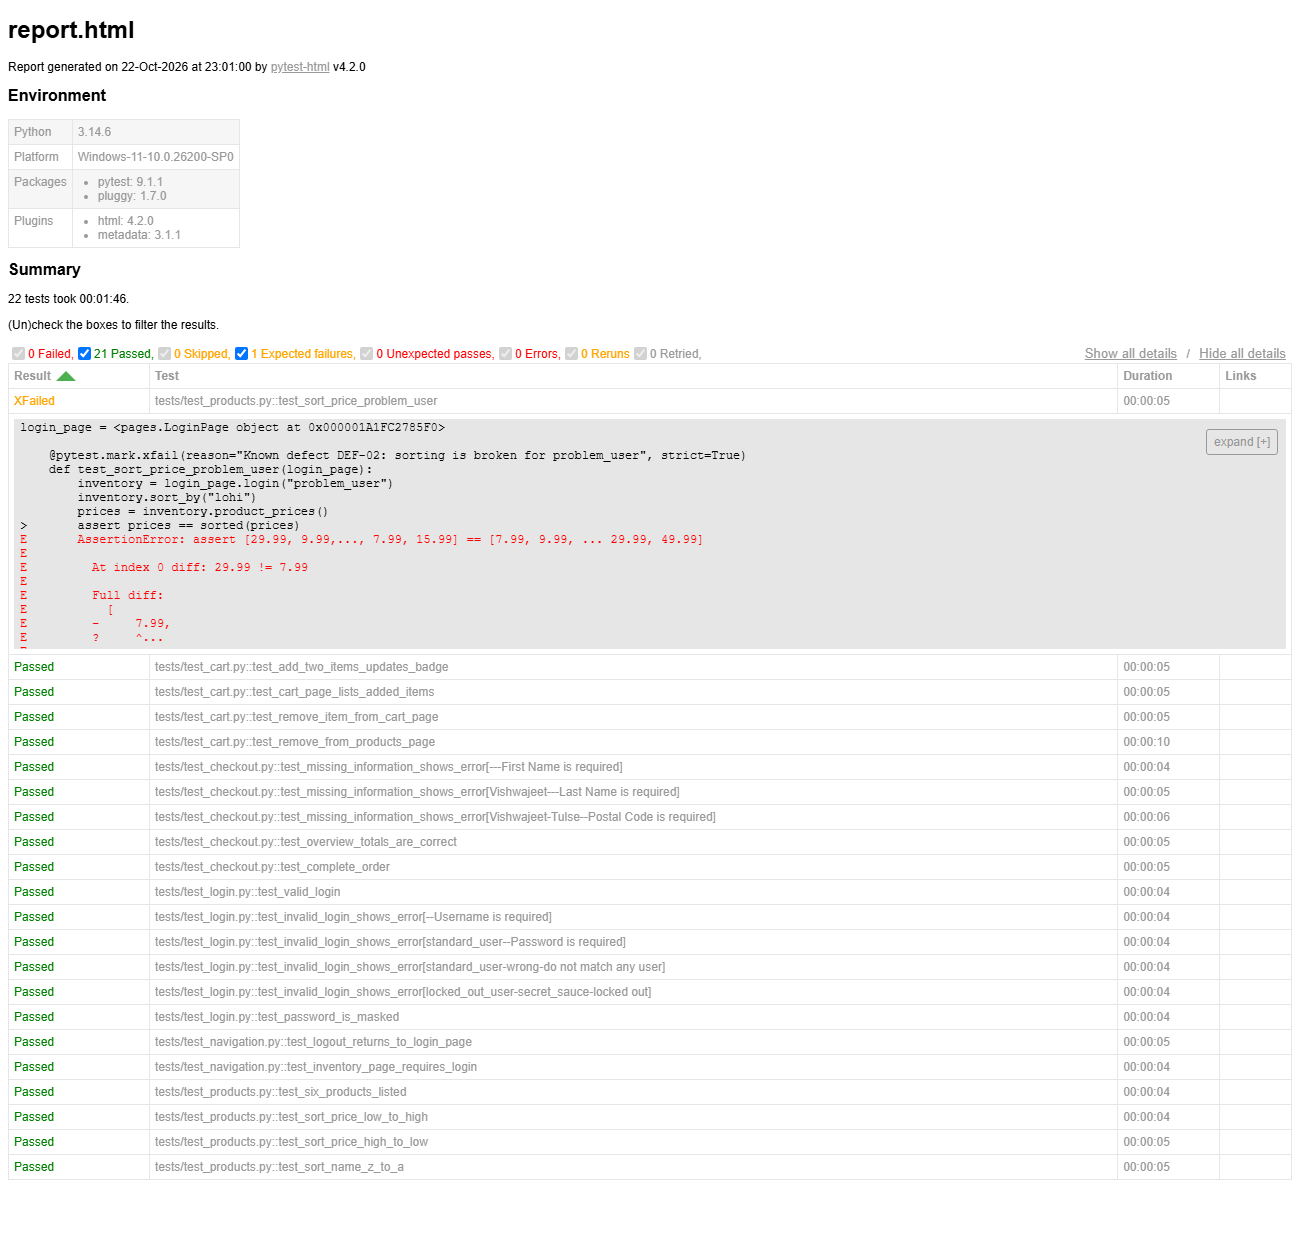
\includegraphics[width=0.95\textwidth]{figures/html_report.png}}
\caption{pytest-html report of the final run}
\label{fig:htmlreport}
\end{figure}
\begin{figure}[H]
\centering
\fbox{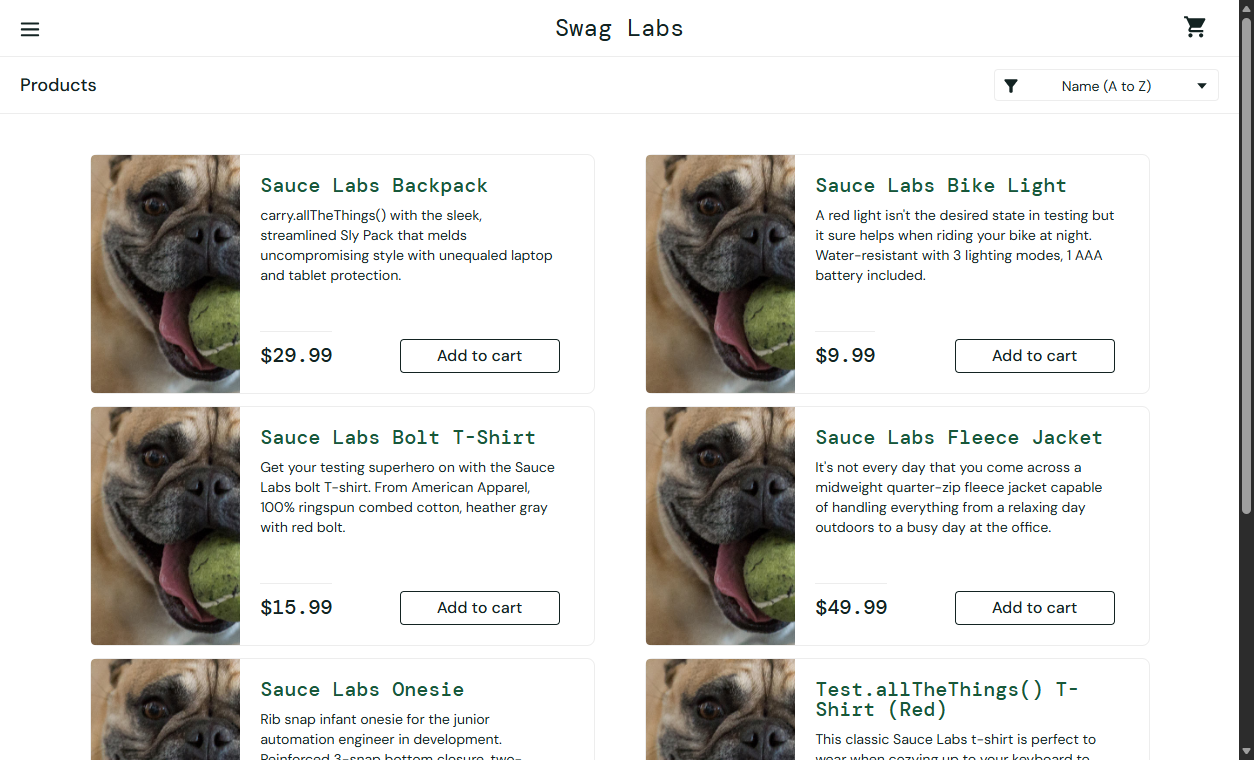
\includegraphics[width=0.8\textwidth]{../reports/screenshots/test_sort_price_problem_user.png}}
\caption{Screenshot captured automatically when the expected-failure test is forced to run: prices are not sorted for problem\_user}
\label{fig:failshot}
\end{figure}

\section{Outputs}
\begin{itemize}
  \item \texttt{reports/report.html}: self-contained HTML report (21 passed, 1 xfailed).
  \item \texttt{reports/console\_output.txt}: console log of the run.
  \item \texttt{reports/screenshots/}: PNG captured for each failed test.
  \item Execution time: 105.6 s for 22 tests in headless Edge, versus about two hours for the same cases executed manually.
\end{itemize}

% =====================================================================
\chapter{Deployment and Maintenance}
\section{Installation and un-installation}
\begin{lstlisting}
git clone https://github.com/VishwajeetTulse/ecommerce-automation-testing
cd ecommerce-automation-testing
pip install -r requirements.txt        # selenium, pytest, pytest-html
python -m pytest                       # run everything, headless Edge
\end{lstlisting}
Selenium Manager downloads the matching browser driver automatically. To un-install, delete the folder and \texttt{pip uninstall selenium pytest pytest-html}.

\section{User help}
\begin{lstlisting}
python -m pytest --headed                 # watch the browser
python -m pytest --browser chrome         # use Chrome
python -m pytest tests/test_checkout.py   # one module
python -m pytest -k sort                  # tests whose name contains "sort"
\end{lstlisting}
Open \texttt{reports/report.html} after the run. If a test fails, look at its screenshot in \texttt{reports/screenshots/}; if the site's DOM changed, update the locator in \texttt{tests/pages.py} only.

% =====================================================================
\chapter{Conclusion and Future Scope}
This mini project automated the regression test cases of an e-commerce website with Selenium WebDriver, Python and pytest. A small Page Object Model keeps locators out of the tests, fixtures give every test an isolated browser, parametrisation covers several data sets with one function, and an HTML report with automatic screenshots makes failures easy to diagnose. The final suite of 22 tests runs unattended in under two minutes and currently passes except for one documented defect kept as an expected failure.

Future scope: run the suite in a CI pipeline (GitHub Actions) on every commit, add cross-browser runs on Selenium Grid, extend coverage to the remaining special users, add API-level checks, and integrate with a test-management tool for traceability to the manual test cases.

% =====================================================================
\begin{thebibliography}{99}
\bibitem{garousi2016} V. Garousi and M. V. M\"antyl\"a. 2016. When and what to automate in software testing? A multi-vocal literature review. \emph{Information and Software Technology} 76 (2016), 92--117.
\bibitem{leotta2013} M. Leotta, D. Clerissi, F. Ricca and C. Spadaro. 2013. Improving test suites maintainability with the Page Object pattern: an industrial case study. In \emph{Proc. ICST Workshops}. IEEE, 108--113.
\bibitem{leotta2014} M. Leotta, D. Clerissi, F. Ricca and P. Tonella. 2014. Visual vs. DOM-based web locators: an empirical study. In \emph{Proc. International Conference on Web Engineering (ICWE)}. Springer, 322--340.
\bibitem{bruns2009} A. Bruns, A. Kornstadt and D. Wichmann. 2009. Web application tests with Selenium. \emph{IEEE Software} 26, 5 (2009), 88--91.
\bibitem{ramya2017} P. Ramya, V. Sindhura and P. V. Sagar. 2017. Testing using Selenium web driver. In \emph{Proc. 2nd International Conference on Electrical, Computer and Communication Technologies (ICECCT)}. IEEE, 1--7.
\bibitem{rafi2012} D. M. Rafi, K. R. K. Moses, K. Petersen and M. V. M\"antyl\"a. 2012. Benefits and limitations of automated software testing: systematic literature review and practitioner survey. In \emph{Proc. 7th International Workshop on Automation of Software Test (AST)}. IEEE, 36--42.
\bibitem{berner2005} S. Berner, R. Weber and R. K. Keller. 2005. Observations and lessons learned from automated testing. In \emph{Proc. 27th International Conference on Software Engineering (ICSE)}. ACM, 571--579.
\bibitem{seleniumdocs} Selenium Project. \emph{Selenium WebDriver Documentation}. \url{https://www.selenium.dev/documentation/webdriver/}
\bibitem{pytestdocs} pytest Developers. \emph{pytest Documentation}. \url{https://docs.pytest.org/}
\bibitem{saucedemo} Sauce Labs. \emph{Swag Labs sample application}. \url{https://www.saucedemo.com}
\bibitem{bookPressman} R. S. Pressman. 2010. \emph{Software Engineering: A Practitioner's Approach} (7th ed.). McGraw-Hill.
\end{thebibliography}

% =====================================================================
\begin{appendices}

\chapter{Laboratory assignments on Project Analysis of Algorithmic Design}
\begin{itemize}
\item \textbf{IDEA Matrix.} Increase: regression frequency. Drive: fast feedback to developers. Educate: students on WebDriver and pytest. Accelerate: a two-hour manual run to two minutes. Improve: diagnosability through screenshots. Deliver: one-command suite and report. Evaluate: pass/fail per module. Associate: automated tests with manual case IDs. Ignore: visual pixel checks. Decrease: duplicated locators. Eliminate: fixed sleeps. Avoid: inter-test dependencies.
\item \textbf{Feasibility.} Execution is $O(n)$ in the number of tests; each test performs a constant number of browser actions. No NP-hard component.
\item \textbf{Function.} $x$ = (test, data set), $y = f(x) \in \{\mathrm{pass}, \mathrm{fail}, \mathrm{xfail}\}$, with $f$ evaluated by executing the test's assertions against the live application.
\end{itemize}

\chapter{Laboratory assignments on Project Quality and Reliability Testing of Project Design}
\begin{itemize}
\item \textbf{Objects and morphisms.} Objects: WebDriver, LoginPage, InventoryPage, CartPage, CheckoutPage, Test, Report. Morphisms: open (driver $\to$ LoginPage), login (LoginPage $\to$ InventoryPage), go\_to\_cart (InventoryPage $\to$ CartPage), checkout (CartPage $\to$ CheckoutPage), execute (Test $\to$ verdict). The page-object methods compose: $\mathrm{checkout} \circ \mathrm{go\_to\_cart} \circ \mathrm{login} \circ \mathrm{open}$.
\item \textbf{Functional dependency graph.} Tests depend on fixtures (\texttt{driver} $\to$ \texttt{login\_page} $\to$ \texttt{inventory} $\to$ \texttt{checkout}); fixtures depend on page objects; page objects depend on Selenium. See Fig.\ref{fig:arch-dig}.
\item \textbf{Test data.} Parametrised sets for login (4) and checkout validation (3); product slugs \texttt{sauce-labs-backpack}, \texttt{sauce-labs-bike-light}, \texttt{sauce-labs-onesie}; expected amounts 39.98 / 3.20 / 43.18.
\item \textbf{Black-box test cases.} Listed in Table \ref{tab:tests}; each corresponds to a manual test case of the companion project.
\end{itemize}

\chapter{Project Planner}
\label{app:plan}
\begin{table}[H]
\begin{center}
\def\arraystretch{1.3}
\begin{tabularx}{\textwidth}{| c | X | c | c |}
\hline
Week & Activity & Deliverable & Status \\ \hline
1 & Install Python, Selenium, pytest; first script; select manual cases to automate & Environment, case list & Done \\ \hline
2 & Page objects, driver fixture, login and products tests & \texttt{pages.py}, \texttt{conftest.py}, 2 test files & Done \\ \hline
3 & Cart, checkout, navigation tests; xfail; HTML report; screenshot hook & 5 test files, \texttt{pytest.ini} & Done \\ \hline
4 & Full runs, fix login default-argument defect, README, repository, report & report.html, report.pdf & Done \\ \hline
\end{tabularx}
\end{center}
\caption{Project planner}
\end{table}

\chapter{Reviewers Comments of Paper Submitted}
Not applicable for this mini project.

\chapter{Plagiarism Report}
To be attached after checking through the institute's plagiarism tool.

\chapter{Term-II Project Laboratory Assignments}
\begin{enumerate}
\item Review of design: the guide's suggestion to keep page objects minimal and avoid a heavy framework was followed.
\item Project workstation: Windows 11 laptop with Python 3.14, Selenium 4.51, pytest 9, Microsoft Edge 142, VS Code and Git; Selenium Manager handled the driver.
\item Programming: completed as described in Chapter 8.
\item Testing: final run 21 passed, 1 xfailed in 105.6 s; report and screenshots in Chapter 10.
\end{enumerate}

\chapter{Information of Project Group Members}
\begin{enumerate}
\item Name : Vishwajeet Tulse
\item Date of Birth :
\item Gender :
\item Permanent Address :
\item E-Mail :
\item Mobile/Contact No. :
\item Placement Details :
\item Paper Published : --
\end{enumerate}
\newpage
\begin{enumerate}
\item Name : Student Name 2
\item Date of Birth :
\item Gender :
\item Permanent Address :
\item E-Mail :
\item Mobile/Contact No. :
\item Placement Details :
\item Paper Published : --
\end{enumerate}
\newpage
\begin{enumerate}
\item Name : Student Name 3
\item Date of Birth :
\item Gender :
\item Permanent Address :
\item E-Mail :
\item Mobile/Contact No. :
\item Placement Details :
\item Paper Published : --
\end{enumerate}
\newpage
\begin{enumerate}
\item Name : Student Name 4
\item Date of Birth :
\item Gender :
\item Permanent Address :
\item E-Mail :
\item Mobile/Contact No. :
\item Placement Details :
\item Paper Published : --
\end{enumerate}
\end{appendices}

\end{document}
